
\thispagestyle{fancy}


\section{Rekombinationsmechanismen}
%
\begin{figure}[h]
\centering
\begin{minipage}[t]{1\linewidth}
\centering
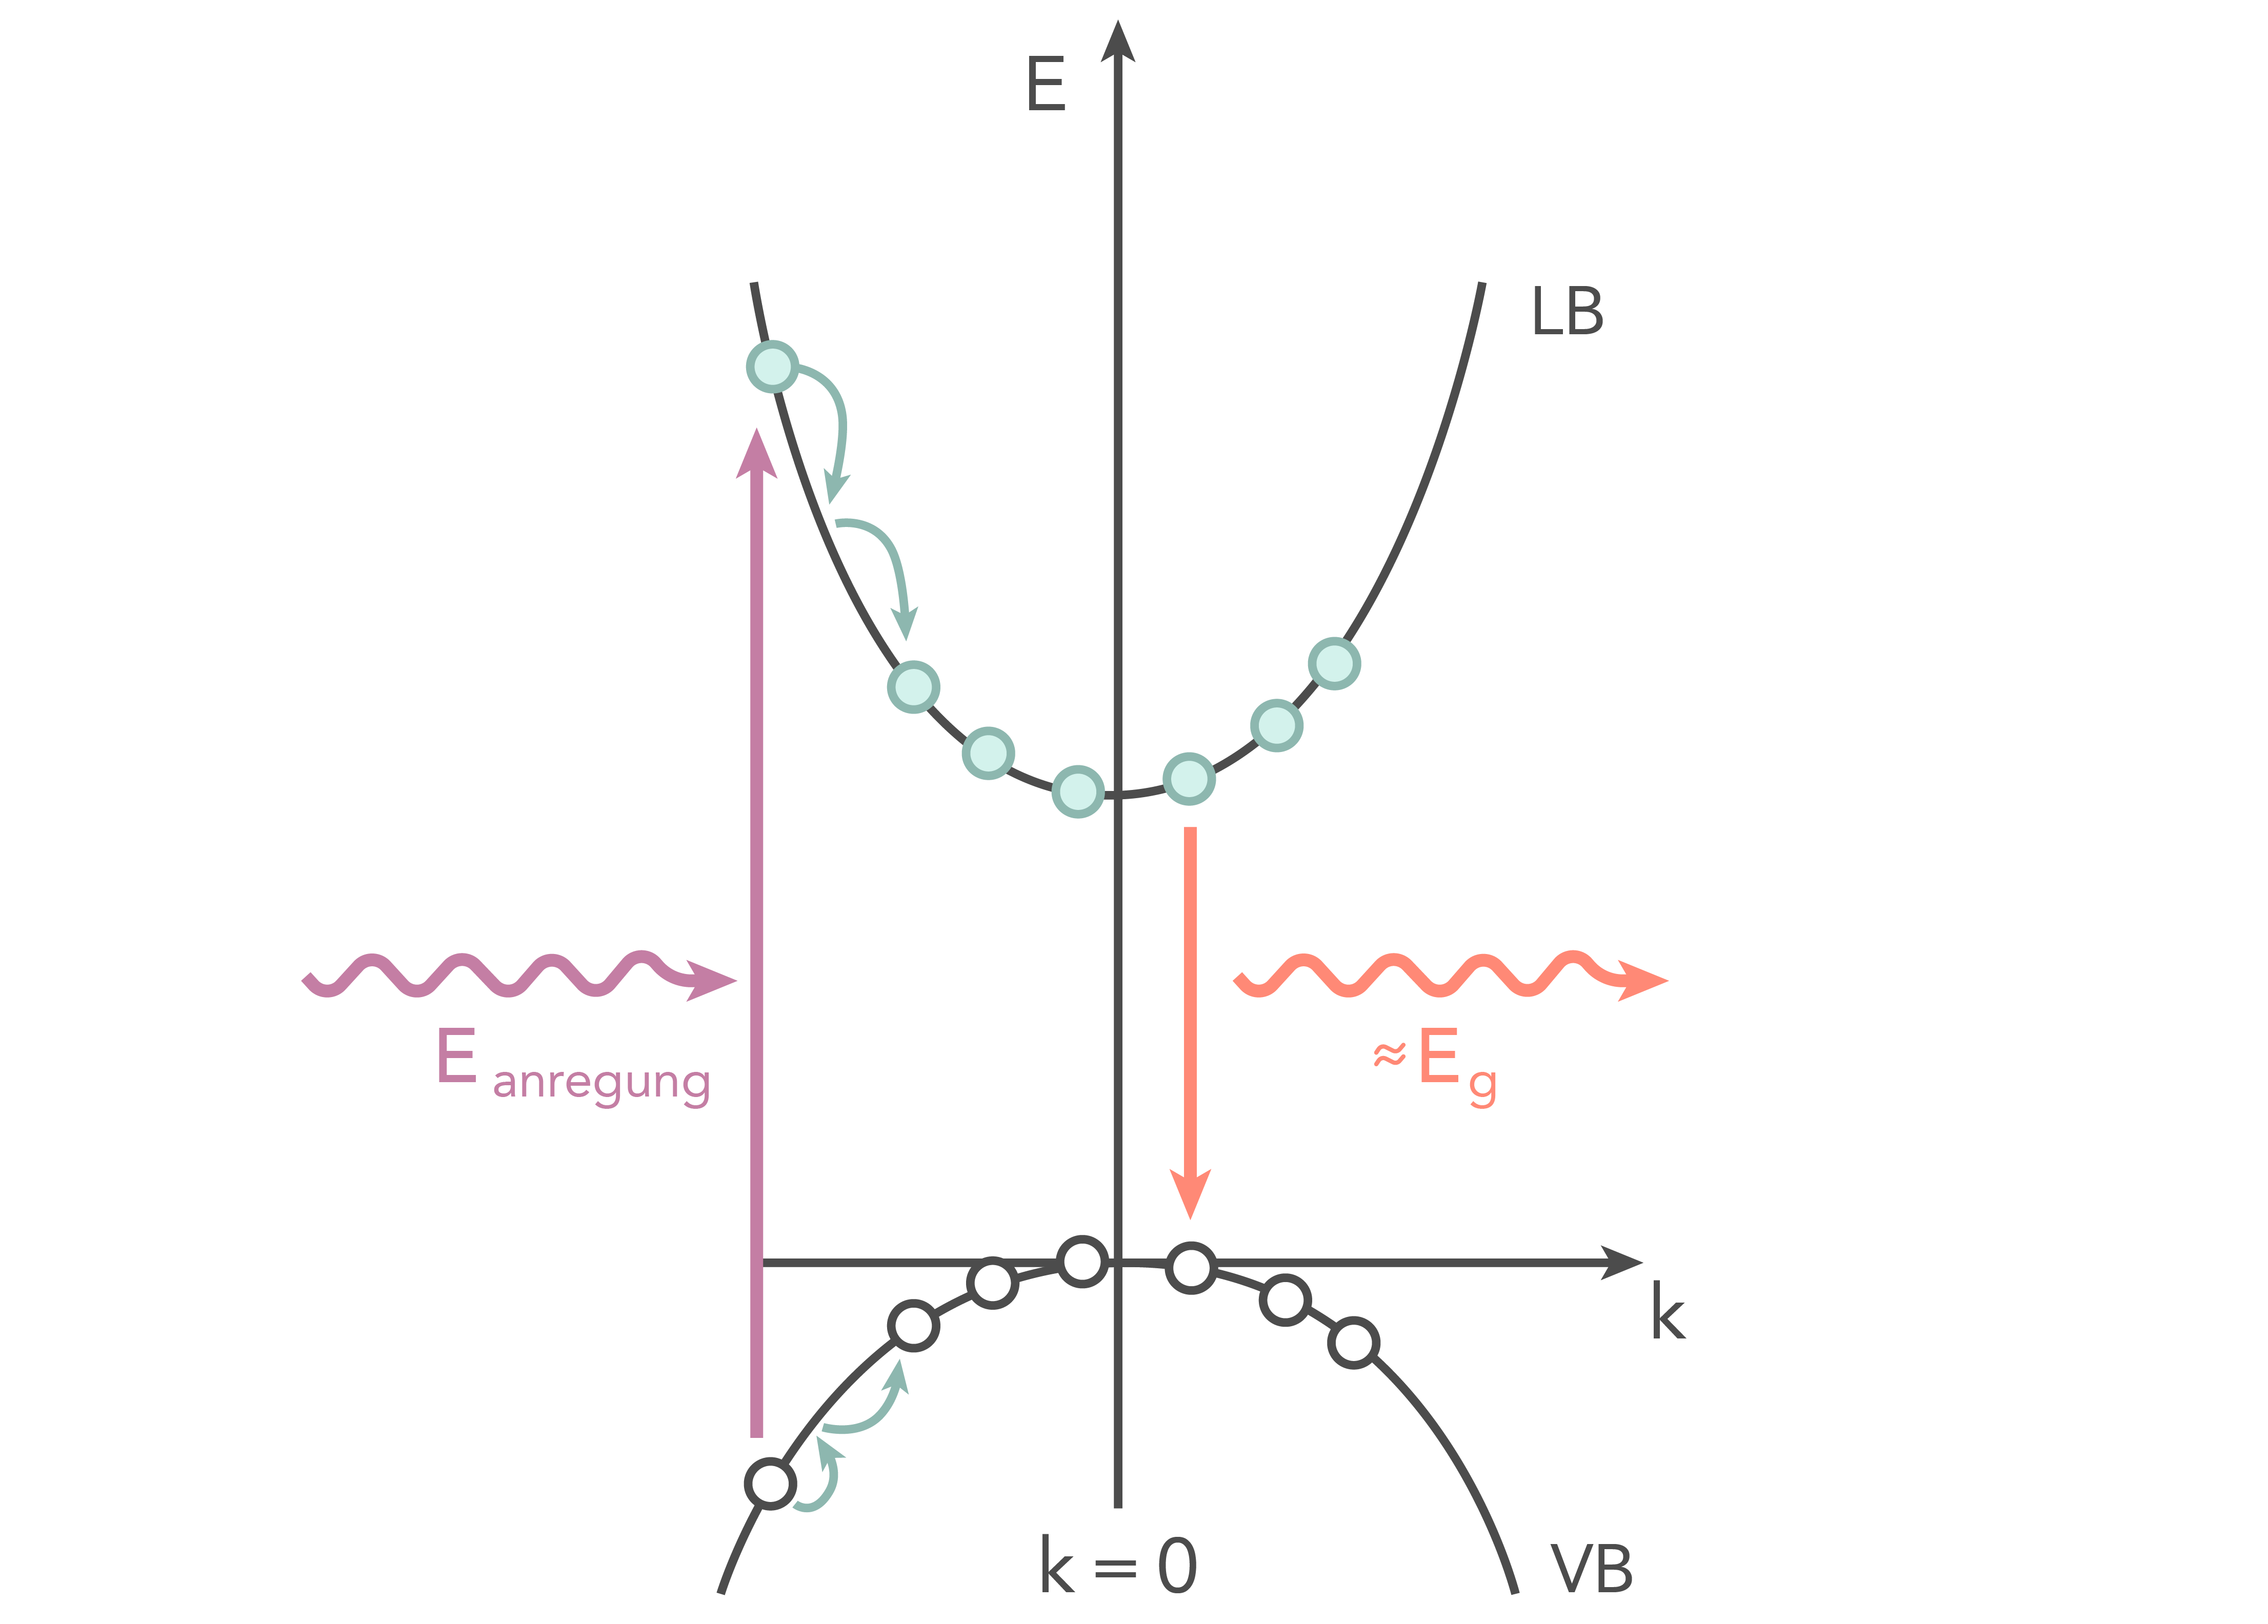
\includegraphics[width=0.8\linewidth]{Bilder/bandrekomb.png}
\end{minipage}% <- sonst wird hier ein Leerzeichen eingefügt
\caption{Durch Einstrahlung eines Photons mit ausreichender Energie können Elektronen vom Valenzband in das Leitungsband angeregt werden. Von dort aus rekombinieren Elektronen und Loch entweder strahlend unter Aussendung eines Photons oder nicht-strahlend.}
 \label{fig:bandrekomb}
\end{figure}
\noindent
In der Photolumineszenzspektroskopie wird Licht als Anregungsquelle von Halbleitermaterialien für die Erzeugung eines Elektron-Loch-Paars benutzt. Dabei wird ein Elektron aus dem Valenzband in das Leitungsband angehoben und ein Loch zurückgelassen wie in Abbildung \ref{fig:bandrekomb} dargestellt ist. Die Elektronen relaxieren anschließend sehr schnell in das Minimum des Leitungsbandes und analog die Löcher in das Minimum des Valenzbandes. 
\newline
Leitungs- und Valenzband befinden sich im Fall von AlGaN am gleichen $\vec{k}$ -Vektor im reziproken Raum, dem sog. $\Gamma$ -Punkt. Das macht das Materialsystem AlGaN zu einem direkten Halbleiter, was von besonderem Vorteil ist. Denn ein direkter Bandübergang ist die wichtigste Grundlage für eine effiziente halbleiterbasierte Lichtquelle. 
\begin{figure}[htb]
    \centering
    \begin{minipage}[t]{0.49\linewidth}
        \centering
        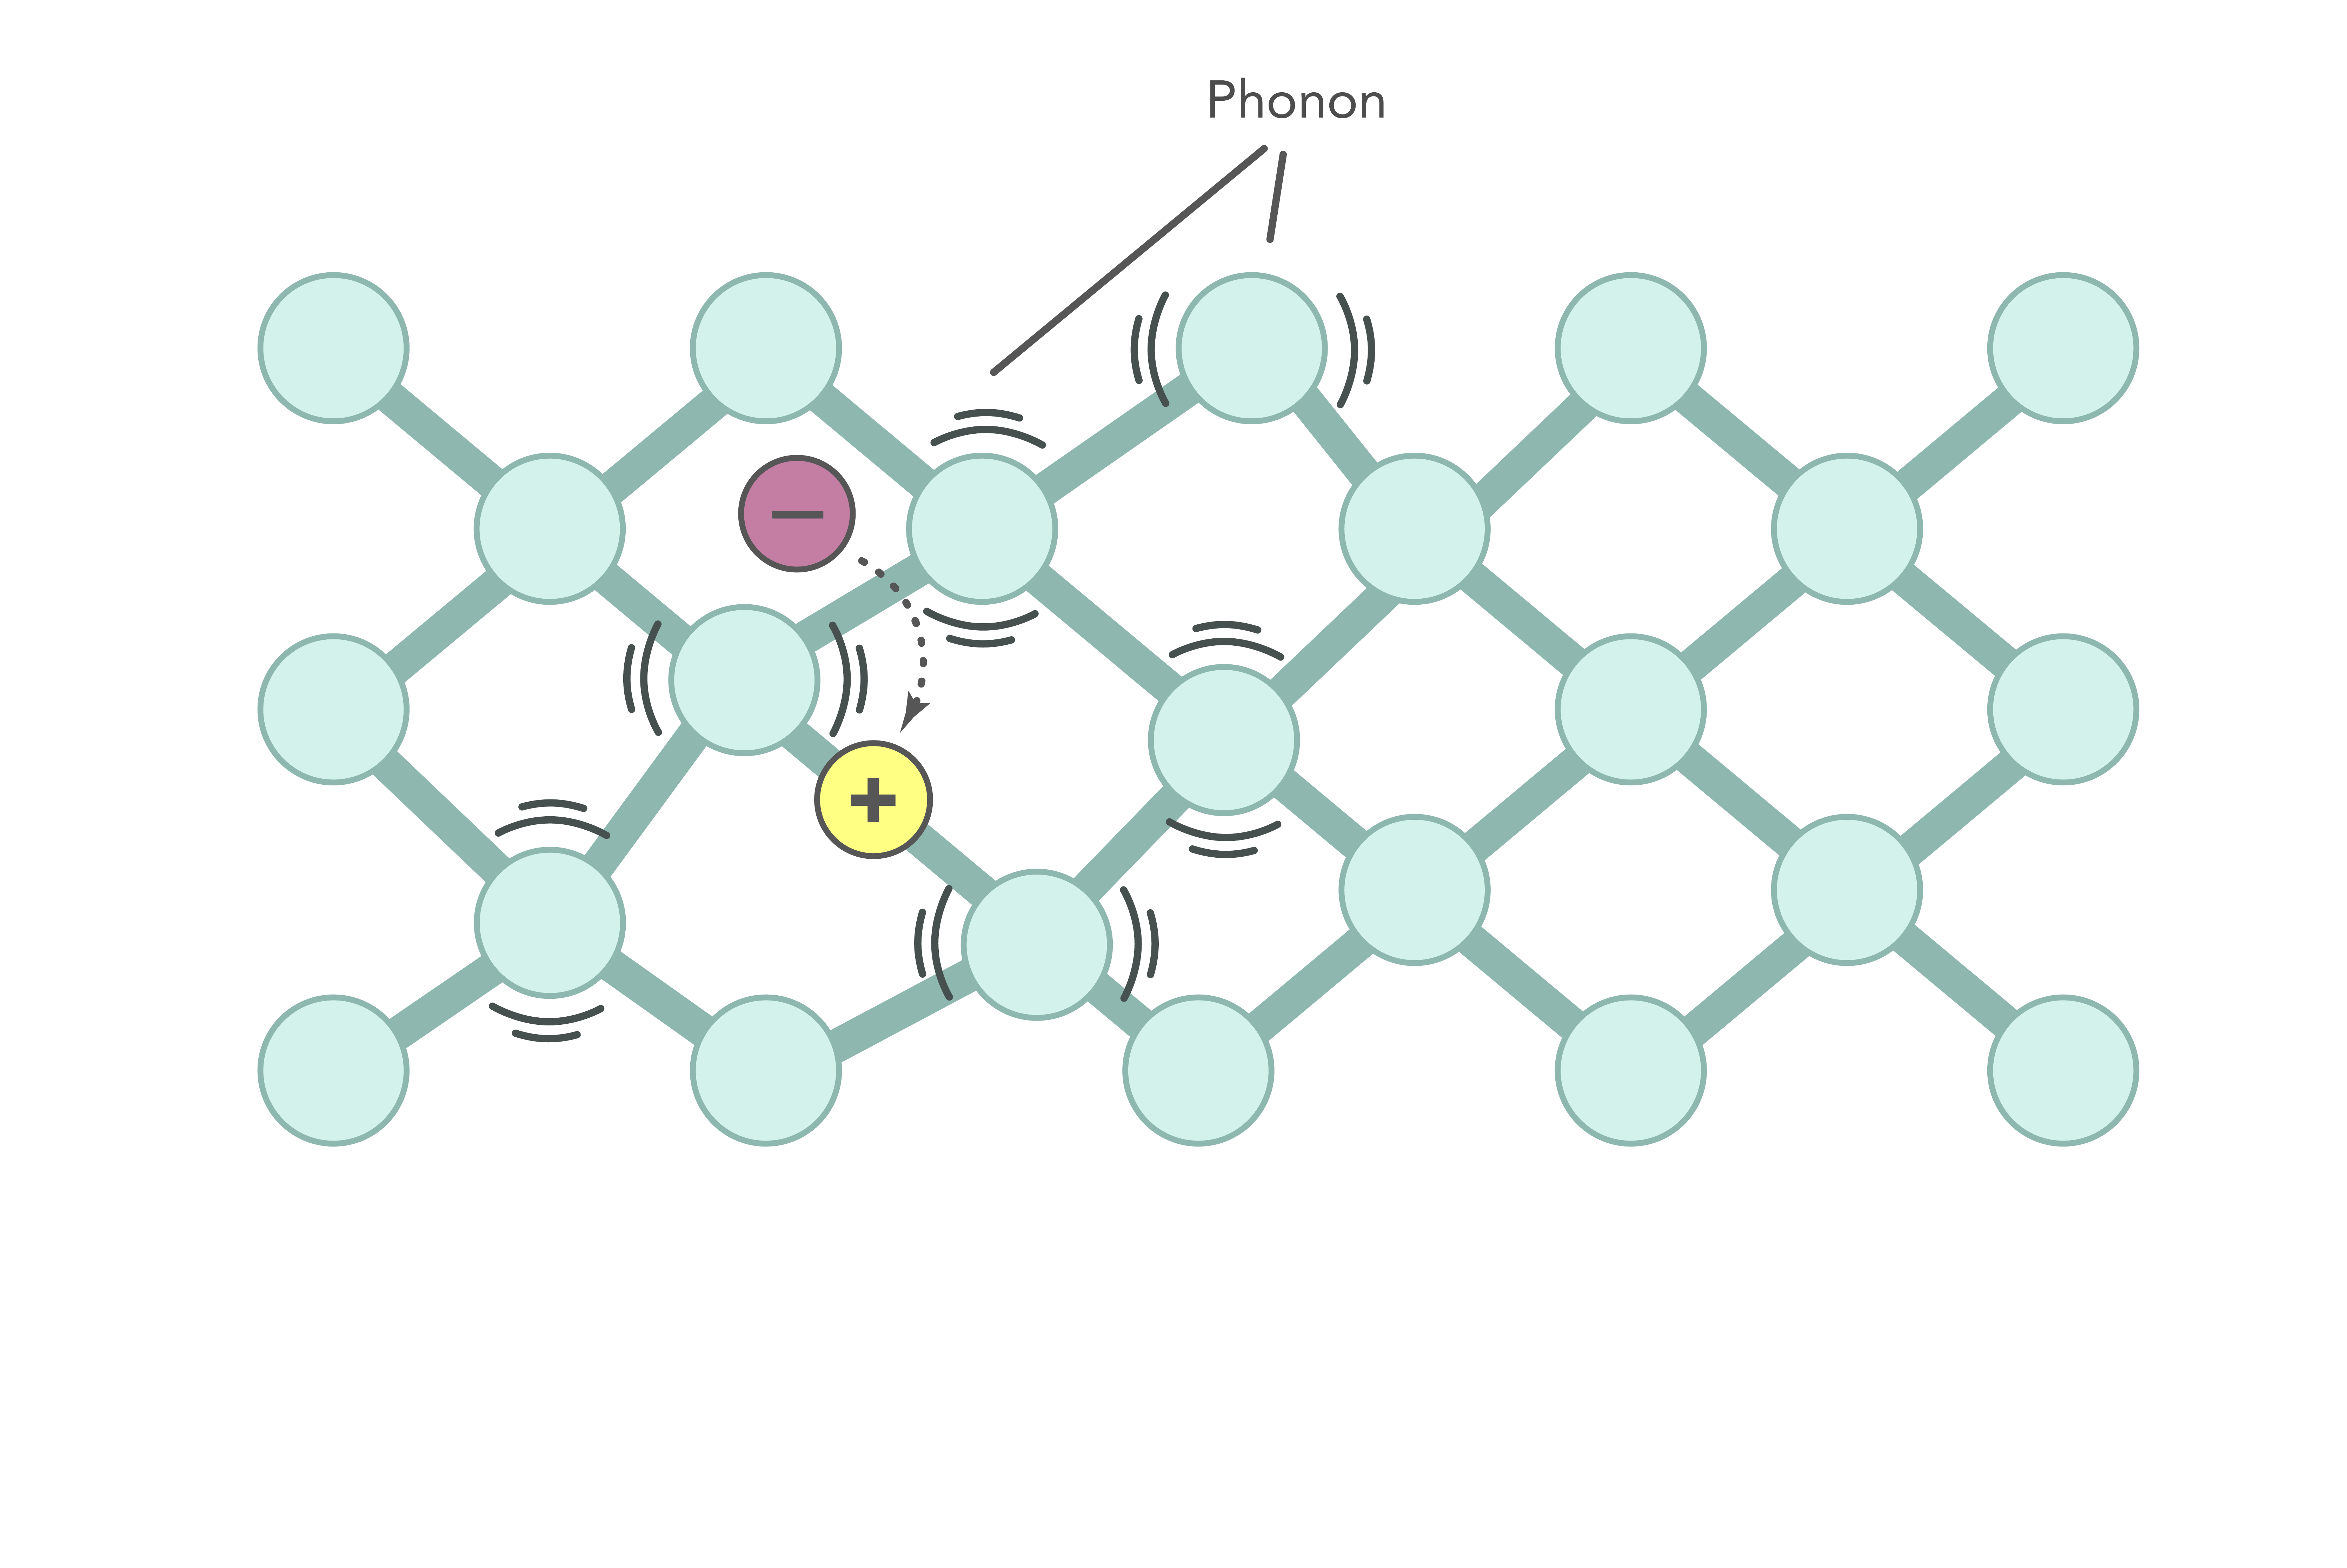
\includegraphics[width=\linewidth]{Bilder/nonradRekomb.png}
        \caption{Rekombination von Elektron und Loch unter Teilnahme eines Phonons.}
				\label{fig:rekombphoton}
    \end{minipage}% <- sonst wird hier ein Leerzeichen eingefügt
    \hfill
    \begin{minipage}[t]{0.49\linewidth}
        \centering
        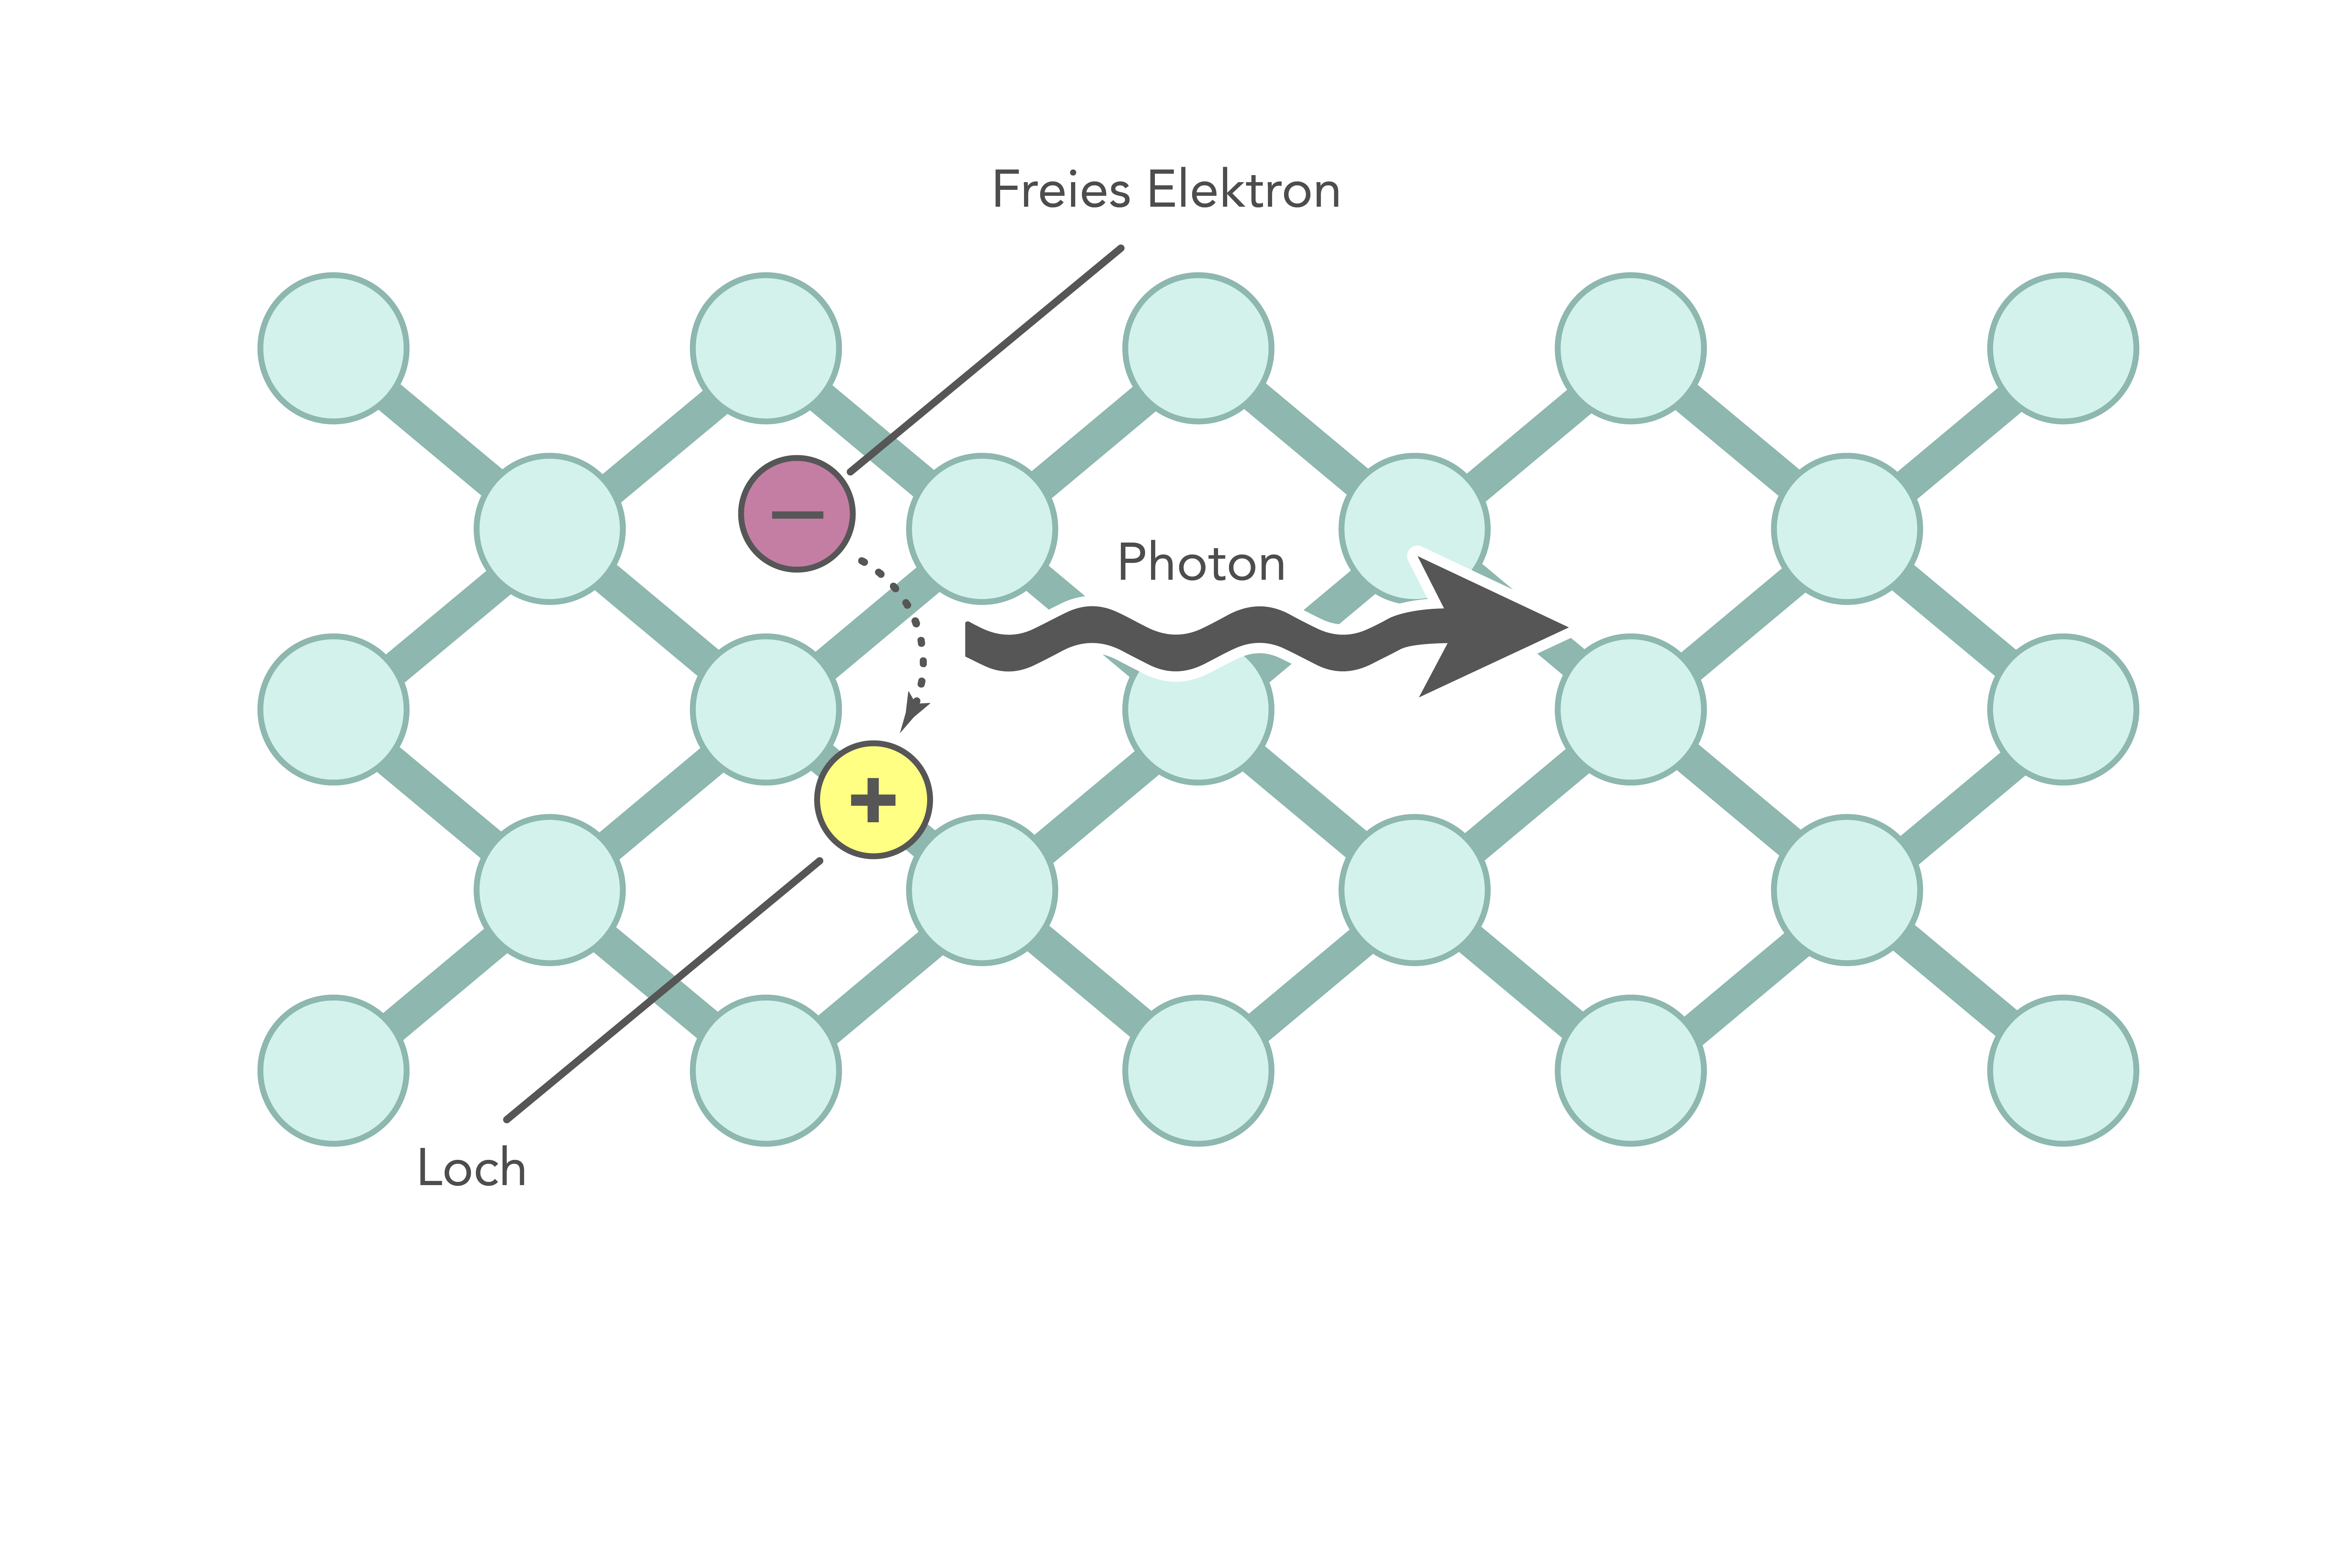
\includegraphics[width=\linewidth]{Bilder/radRekomb.png}
        \caption{Strahlende Rekombination von Elektron und Loch und Aussendung eines Photons}
    \end{minipage}
\end{figure}
\noindent
Denn die Wahrscheinlichkeit einer Anregung und daraufhin folgenden Rekombination unter Aussendung eines Photons ist deutlich höher, da kein Phonon am Prozess beteiligt sein muss (Abb. \ref{fig:rekombphoton}). Die Rekombination kann dennoch auch nicht-strahlend erfolgen, weil epitaktisch gewachsene Halbleitersstrukturen herstellungsbedingt beispielsweise nicht ohne ungewollte Dotierung durch Fremdatome, Versetzungen oder Fehlstellen an Atomgitterplätzen (Vakanzen) gewachsen werden können. Diese fungieren als sogenannte Störstellen und haben diskrete Energieniveaus. 
%
\begin{figure}[h]
    \centering
    \begin{minipage}[t]{0.75\linewidth}
        \centering
        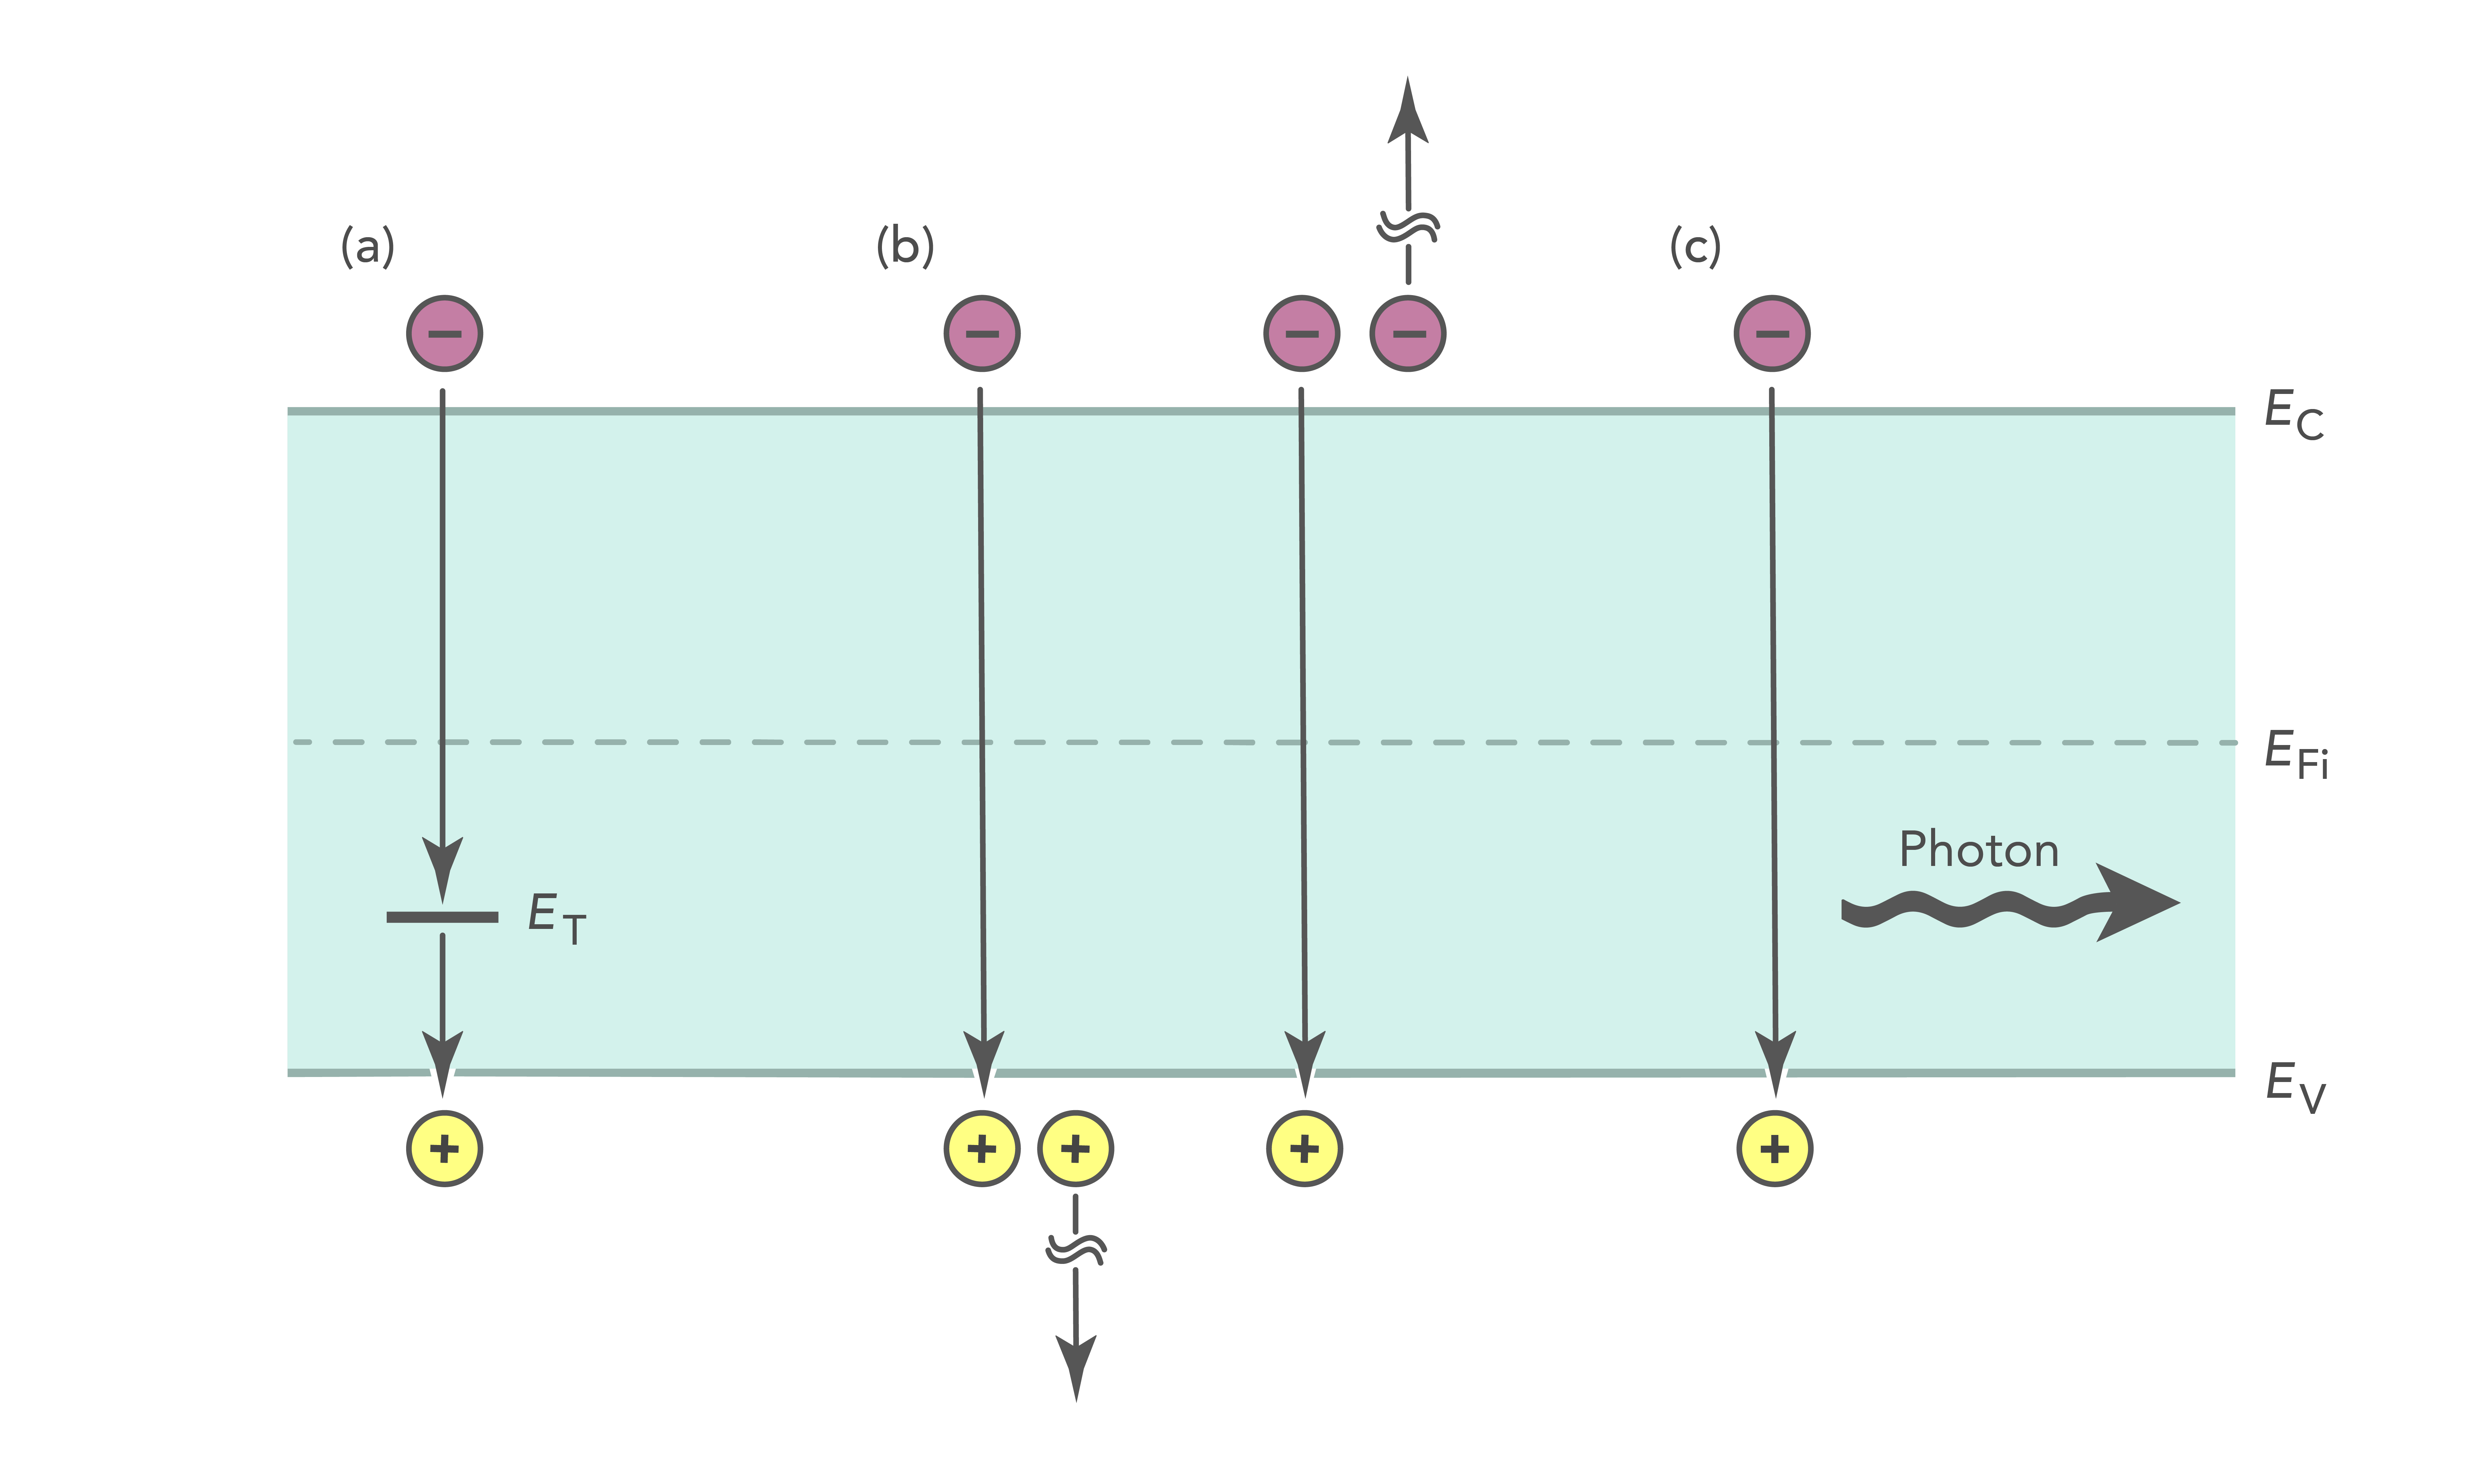
\includegraphics[width=\linewidth]{Bilder/rekbomChannels.png}
        \caption{Übersicht über die beteiligten Rekombinationsprozesse im ABC-Modell, dabei stellt (a) die SRH-Rekombination, (b) die Auger-Rekombination und (c) die strahlende Rekombination dar.}
        \label{fig:rekombChannels}
    \end{minipage}% <- sonst wird hier ein Leerzeichen eingefügt
\end{figure}
\noindent
%
Dazu werden drei Prozesse betrachtet: Zuallererst die nichtstrahlende Rekombination, die durch die Shockley-Read-Hall- (SRH-) Rekombination an Defekten beschrieben und durch den Parameter $A$ berücksichtigt wird ($R_{nonrad} = A \cdot n $). Sie ist linear abhängig von der Ladungsträgerdichte $n$. Sie findet unter der Beteiligung eines Defektniveaus und eines Phonons statt. Der A-Koeffizient ist invers proportional zur SRH-Rekombinations-Lebensdauer. Diese wurde bei defektreichen AlGaN-Schichten im Bereich von einigen $ps$ gemessen. Mit AlGaN-QWs mit Bulk-AlN-Substraten wurden dagegen bereits Lebensdauern im Bereich einiger $ns$ erreicht \cite{1882-0786-4-9-092101} \cite{doi:10.1002/pssc.201100424}.
\newline
Der strahlende Prozess der spontanen Rekombination ist für niedrige Ladungsträgerdichten quadratisch in $n$ und tritt als Zwei-Teilchen Prozess bei dem Loch und Elektron beteiligt sind ($R_{rad} = B \cdot n^2 $) auf. Dieser wird beschrieben mit dem Koeffizienten B. Der B-Koeffizient ist stark abhängig vom Design des MQWs wie z.B. der QW-Dicke, QW-Barrieren-Höhe, Verzerrung des AlGaN-QWs und dem Polarisationsfeld im QW \cite{kneissl}. Typische Werte für den B-Koeffizienten liegen in einem Bereich um $2 \cdot 10^{-11} \thinspace cm^3 \thinspace s^{-1}$ \cite{1882-0786-8-2-022104} \cite{1882-0786-4-5-052101}.  
\newline
Der letzte Prozess ist die Auger-Rekombination, die speziell für sehr hohe Anregungsleistungsdichten relevant ist und dann durch die kubische Abhängigkeit stark dominiert ($R_{auger} = C \cdot n^3 $). Dabei gibt ein bereits in das Leitungsband angeregte Elektron seine Energie an ein weiteres Elektron im Leitungsband ab. Dieses relaxiert dann entweder wieder zum Leitungsbandminimum unter Mitwirkung von Phononen oder verlässt bei Oberflächennähe den Kristall. Der letzte Fall bildet die Grundlage für die Auger-Elektronen-Spektroskopie.
Die Größenordnung des C-Koeffizienten für die Gruppe-III-Materialien ist immer noch in Diskussion \cite{8b1c5cf85d5a45e0ae9acca7b03dc349} \cite{doi:10.1063/1.2785135} \cite{doi:10.1002/pssc.200880950} und die Werte für blau-violette LEDs liegen zwischen $1 \cdot 10^{-31}$ und $2 \cdot 10^{-30} \thinspace cm^6 \thinspace s^{-1}$. Die Messmethoden um den C-Koeffizienten für UV-LEDs zu bestimmen sind noch ungenauer \cite{1882-0786-8-2-022104}. Theoretische Modelle sagen aber voraus, dass der C-Koeffizient kleiner werden sollte mit kleiner werdender Wellenlänge \cite{doi:10.1063/1.3570656}.
\newline
Die effektive Rekombination ist somit die Summe aus der strahlenden Rekombination, der nicht-strahlenden Rekombination und der Auger-Rekombination.
\begin{equation}
    R_{eff} = R_{rad} + R_{nonrad} + R_{auger}
    \label{eq:iqe1}
\end{equation}
Der allgemein verwendete Ansatz zur Beschreibung der effektiven Rekombinationsrate $R_{eff}$ (oder auch Generationsrate $G$) wird mit Hilfe der genannten Koeffizienten beschrieben. Er beruht auf der Abhängigkeit der beteiligten Prozesse von der Ladungsträgerdichte $n$ und wird daher auch als ABC-Modell bezeichnet.
\begin{equation}
    R_{eff} (G) = A \cdot n + B \cdot n^2 + C \cdot n^3 
    \label{eq:iqe2}
\end{equation}
Weiter wird angenommen, dass die Anregungsleistungsdichte des Lasers P proportional zu
der Ladungsträger-Generationsrate G ist. Die strahlende Rekombination $R_{rad}$ wird hauptsächlich durch den Überlapp der Wellenfunktionen von Elektronen und Loch im Leitungsband und Valenzband des QW beeinflusst. Dieser wiederum ist stark abhängig vom QCSE (Abb. 
\ref{fig:qcse}) und besonders bedeutend bei heteroepitaktisch gewachsenen Halbleiterstrukturen. 
%
